%Auteurs : Nicolas Englebert
\documentclass[british,french,11pt, a4paper, openany]{book}

% Règles de bonne pratiques :
% https://fr.wikibooks.org/wiki/LaTeX/Gestion_des_gros_documents
\usepackage{../../Builder/preambule}
% %%%%%%%%%%%%%%%%
%%% Packages %%%
%%%%%%%%%%%%%%%%

%%% Compatibilité %%%
\begingroup\expandafter\expandafter\expandafter\endgroup
\expandafter\ifx\csname IncludeInRelease\endcsname\relax
\usepackage{fixltx2e}
\fi 					% Si version LaTeX < 2015, inclut un fix.

%%% Général %%%
\usepackage[utf8]{inputenc}
\usepackage{babel}
\usepackage{lmodern}
\usepackage[T1]{fontenc}
\addto\extrasfrench{\sisetup{locale = FR,detect-all}} % Switch siunitx en fonction de la langue babel :)
\addto\extrasbritish{\sisetup{locale = UK,detect-all}}
\usepackage{courier}
\usepackage{graphicx}
%\usepackage{cancel}

%%% Tableau %%%
%\usepackage{tabularx} %Permet d'auto dimensionner les tableaux



%%% Bibliographie %%%
%\usepackage[style=alphabetic,backend=biber]{biblatex}
\usepackage[autostyle]{csquotes}
%\DeclareNameAlias{sortname}{last-first}
%\DeclareFieldFormat{url}{\space\url{#1}}
%\DeclareNameAlias{labelname}{last-first}
%\addbibresource{sample.bib}


%%% Graphiques %%%
%\usepackage{tikz}
%\usepackage{pgfplots}
%\usepackage{circuitikz}

%%% Mise en page %%%
\usepackage{mathtools}
\usepackage{amssymb}
\usepackage{bbm}
\usepackage{amsthm}
%\usepackage[tt]{titlepic}% Centre le titre
%\usepackage{fancyhdr}   % Permet de modifier l'entête & footer
\usepackage{caption}     % Permet d'ajouter des légendes en images sans les mettre en float + dans la marge + ref vers le haut de l'envirronement
\usepackage{wrapfig}
\usepackage{fullpage}
%\usepackage{multicol}   % pour les liste sur plusieurs colonnes
%\usepackage{subfigure}  % alligne deux images cote a cote
\usepackage{float}      %permet de mettre du texte entre les figures grace a [H]. Génial! 
\usepackage{eso-pic}    % Fond d'écran page de garde
\usepackage{adjustbox}  % Empêche les box de sortir de la page


%%% Math %%%
%\usepackage{delarray} % Belles matrices
\usepackage{siunitx}


%%% Codes %%%
%\usepackage{listings}
%\usepackage[final]{pdfpages} %% Inclusion fichier pdf

%% Reference
\usepackage{hyperref}
%\renewcommand*{\figureautorefname}{fig.}
%\def\appendixautorefname{annexe}
%\def\tableautorefname{tab.}
%\renewcommand*{\chapterautorefname}{ch.}
%\newcommand{\subfigureautorefname}{\figureautorefname}



%%%%%%%%%%%%%%%%%
%%% Commandes %%%
%%%%%%%%%%%%%%%%%

%%% Physique %%%
\newcommand{\cst}{\text{cst}}
\newcommand{\D}{\partial}
\newcommand{\E}{\vec E}
\newcommand{\B}{\vec B}
\newcommand{\F}{\vec F}
\newcommand{\modu}[1]{|$#1$|}

%%% Math %%%
\newcommand{\oiint}{\int\!\!\!\!\!\!\! \:\!\subset\!\!\supset\!\!\!\!\!\!\!\int}
\newcommand{\rot}{\operatorname{\vec{rot}}}
\newcommand{\divv}{\operatorname{div}}
\newcommand{\phas}[1]{\underline{#1}}
\newcommand{\RE}{\text{Re}}
\newcommand{\ft}{\overset{\mathcal{F}}{\longleftrightarrow}}
\newcommand{\lt}{\overset{\mathcal{L}}{\longleftrightarrow}}
\newcommand{\DS}{\displaystyle}
\newcommand{\Tr}{\operatorname{Tr}}



%% Box
\shorthandon{:}
\newcommand{\theor}[1]{\adjustbox{minipage=\linewidth-2\fboxsep-2\fboxrule,fbox}{\textsc{\iflanguage{british}{Theorem}{Théorème}: }#1}}
\newcommand{\defi}[1]{\adjustbox{minipage=\linewidth-2\fboxsep-2\fboxrule,fbox}{\textsc{\iflanguage{british}{Definition}{Définition}: }#1}}
\newcommand{\lemme}[1]{\adjustbox{minipage=\linewidth-2\fboxsep-2\fboxrule,fbox}{\textsc{\iflanguage{british}{Lemma}{Lemme}: }#1}}
\newcommand{\prop}[1]{\adjustbox{minipage=\linewidth-2\fboxsep-2\fboxrule,fbox}{\textsc{\iflanguage{british}{Property}{Propriété}}\\ #1}}
\newcommand{\proposition}[1]{\adjustbox{minipage=\linewidth-2\fboxsep-2\fboxrule,fbox}{\textsc{Proposition}\\#1}}
\newcommand{\cadre}[1]{\adjustbox{minipage=\linewidth-2\fboxsep-2\fboxrule,fbox}{#1}}
\newcommand{\retenir}[1]{\adjustbox{minipage=\linewidth-2\fboxsep-2\fboxrule,fbox}{\textbf{\textit{\textsc{\iflanguage{british}{To remember}{À retenir}}: }}#1}}

\newcommand{\corollaire}[1]{\bigbreak\begin{tabular}{||c}
	\begin{minipage}{\textwidth}
		\textsc{\iflanguage{british}{Corollary}{Corollaire}: } \textit{#1}
	\end{minipage}
	\end{tabular}}
\newcommand{\exemple}[1]{\bigbreak\begin{tabular}{|c}
	\begin{minipage}{\textwidth}
		\textsc{\iflanguage{british}{Example}{Exemple}: } #1
	\end{minipage}%
	\end{tabular}}%
\shorthandoff{:}
    

%\pagestyle{headings} % Titre du ch et numéro page dans l'entete
%\renewcommand{\proofname}{Démonstration}
%\addto\captionsfrench{\def\tablename{Tableau}}


%%% Background %%%
\newcommand\BackgroundPic{%
	\put(0,0){%
		\parbox[b][\paperheight]{\paperwidth}{%
			\vfill
			\centering
			\includegraphics[width=\paperwidth,height=\paperheight,%
			keepaspectratio]{../../Builder/ulb.jpg}%
			\vfill
}}}

%%% Annexes Cedu %%%
%\usepackage{calrsfs}
%\DeclareMathAlphabet{\pazocal}{OMS}{zplm}{m}{n}
\usepackage{fourier-orns}

\setlength{\parindent}{0pt} 

%%% Attributs %%%
\newcommand*{\NomduCours}[2]{\def\cours{#1}\def\memo{#2}}
\newcommand*{\annee}[2]{\def\adebut{#1}\def\afin{#2}}

\newcounter{auteurcnt}
\newcommand\addauteur[2]{%
	\stepcounter{auteurcnt}%
	\csdef{auteur\theauteurcnt}{\mbox{#1~\textsc{#2}}}}
\newcommand\getauteur[1]{%
	\csuse{auteur#1}}

\newcounter{illustrateurcnt}
\newcommand\addillustrateur[2]{%
	\stepcounter{illustrateurcnt}%
	\csdef{illustrateur\theillustrateurcnt}{\mbox{#1~\textsc{#2}}}}
\newcommand\getillustrateur[1]{%
	\csuse{illustrateur#1}}

\newcounter{rappeltheocnt}
\newcommand\addrappeltheo[2]{%
	\stepcounter{rappeltheocnt}%
	\csdef{rappeltheo\therappeltheocnt}{\mbox{#1~\textsc{#2}}}}
\newcommand\getrappeltheo[1]{%
	\csuse{rappeltheo#1}}

\newcounter{professeurcnt}
\newcommand\addprofesseur[2]{%
	\stepcounter{professeurcnt}%
	\csdef{professeur\theprofesseurcnt}{\mbox{#1~\textsc{#2}}}}
\newcommand\getprofesseur[1]{%
	\csuse{professeur#1}}

\newcounter{iter}

% Attributs
\NomduCours{Mécanique rationelle I}{MECA-H-100}
\addauteur{Nicolas}{Englebert}
\addprofesseur{Alain}{Delchambre}
\annee{2013}{2014}

% Document
\begin{document}
\def\equationautorefname~#1\null{%
	(#1)\null
}


%%%%%%%%%%%%%%%%%
% Préliminaires %
%%%%%%%%%%%%%%%%%
\frontmatter
\AddToShipoutPicture*{\BackgroundPic}

\begin{titlepage}
	\begin{center}	
			
		\newcommand{\HRule}{\rule{\linewidth}{0.5mm}}   			            %Titre en gros
		\includegraphics[width=0.55\textwidth]{../../Builder/titlepage/logo.pdf}~\\[1cm]				%Logo
			
			\textsc{\LARGE Université Libre de Bruxelles}\\[1.5cm]
			\textsc{\Large \iflanguage{british}{Summary}{Synthèse}}\\[0.5cm]
			
			\HRule \\[0.4cm]
			{ \huge \bfseries \cours \ \\\memo \\[0.4cm] }
			
			
			\HRule \\[1.5cm]
			\begin{minipage}[t]{0.6\textwidth}
				\begin{flushleft}%\large
					\emph{\iflanguage{british}{Author}{Auteur}\ifnum\theauteurcnt>1 s\fi:}\\
					\whileboolexpr
					{ test {\ifnumcomp{\value{iter}}{<}{\theauteurcnt}} }%
					{\stepcounter{iter}\getauteur{\theiter}\\}
					\setcounter{iter}{0}%
					\ifnum\theillustrateurcnt>0%
					\ \\
					\emph{Illustrations:}\\
					\whileboolexpr
					{ test {\ifnumcomp{\value{iter}}{<}{\theillustrateurcnt}} }%
					{\stepcounter{iter}\getillustrateur{\theiter}\\}%
					\setcounter{iter}{0}%
					\fi%
					\ifnum\therappeltheocnt>0%
					\ \\
					\emph{\iflanguage{british}{Reminders}{Rappels théoriques}:}\\
					\whileboolexpr
					{ test {\ifnumcomp{\value{iter}}{<}{\therappeltheocnt}} }%
					{\stepcounter{iter}\getrappeltheo{\theiter}\\}%
					\setcounter{iter}{0}%
					\fi%
				\end{flushleft}
			\end{minipage}%
			\begin{minipage}[t]{0.25\textwidth}
				%\begin{flushright}
				%\large
				\emph{\iflanguage{british}{Professor}{Professeur}\ifnum\theprofesseurcnt>1 s\fi:}
				\whileboolexpr
				{ test {\ifnumcomp{\value{iter}}{<}{\theprofesseurcnt}} }%
				{\\ \stepcounter{iter}\getprofesseur{\theiter}}%
				\setcounter{iter}{0}%
				%\end{flushright}
			\end{minipage}
			
			\vfill
			
			% Bottom of the page
			{\large \iflanguage{british}{Year}{Année} \adebut~-~\afin}
			
		\end{center}
	\end{titlepage}

\ \\[2cm]
{\Huge \bfseries Appel à contribution}\\[5mm]
\subsection*{Synthèse Open Source}
\begin{wrapfigure}[5]{l}{4.5cm}
	\includegraphics[scale=0.5]{../../Builder/git.png}
\end{wrapfigure}
Ce document est grandement inspiré de l’excellent cours donné 
par \ifnum\theprofesseurcnt=1 \getprofesseur{1} \else\whileboolexpr
{ test {\ifnumcomp{\value{iter}}{<}{\theprofesseurcnt-2}} }%
{\stepcounter{iter}\getprofesseur{\theiter}, }%
\stepcounter{iter}\getprofesseur{\theiter} et \stepcounter{iter}\getprofesseur{\theiter} \fi%
 à l’EPB (École Polytechnique de Bruxelles), faculté de l’ULB (Université 
Libre de Bruxelles). Il est écrit par les auteurs susnommés avec l’aide de tous les autres étudiants 
et votre aide est la bienvenue ! En effet, il y a toujours moyen de l’améliorer surtout que si le 
cours change, la synthèse doit être changée en conséquence. On peut retrouver le code source à l’adresse 
suivante
\begin{center}
	\url{https://github.com/nenglebert/Syntheses}
\end{center}\bigskip
Pour contribuer à cette synthèse, il vous suffira de créer un compte sur \textit{Github.com}. De
légères modifications (petites coquilles, orthographe, ...) peuvent directement être faites sur le
site ! Vous avez vu une petite faute ? Si oui, la corriger de cette façon ne prendra que quelques 
secondes, une bonne raison de le faire ! \bigskip

Pour de plus longues modifications, il est intéressant de disposer des fichiers : il vous 
faudra pour cela installer \LaTeX, mais aussi \textit{git}. Si cela pose problème, nous sommes 
évidemment ouverts à des contributeurs envoyant leur changement par mail ou n’importe quel autre 
moyen.\bigskip

Le lien donné ci-dessus contient aussi un \texttt{README} contenant de plus amples informations, 
vous êtes invités à le lire si vous voulez faire avancer ce projet ! 

\subsection*{Licence Creative Commons}
\begin{wrapfigure}[3]{r}{2.8cm}
	\vspace{-5mm}
	\includegraphics[scale=0.17]{../../Builder/CC}
\end{wrapfigure}
Le contenu de ce document est sous la licence Creative Commons : \textit{Attribution-NonCommercial-ShareAlike 
4.0 International (CC BY-NC-SA 4.0)}. Celle-ci vous autorise à l'exploiter pleinement, compte-
tenu de trois choses :
\begin{enumerate}
	\item \textit{Attribution} ; si vous utilisez/modifiez ce document vous devez signaler le(s) nom(s)
	      de(s) auteur(s).
	\item \textit{Non Commercial} ; interdiction de tirer un profit commercial de l’œuvre sans 
	      autorisation de l'auteur 
	\item \textit{Share alike} ;  partage de l’œuvre, avec obligation de rediffuser selon la même 
	      licence ou une licence similaire
\end{enumerate}
Si vous voulez en savoir plus sur cette licence :
\begin{center}
	\url{http://creativecommons.org/licenses/by-nc-sa/4.0/}
\end{center}

\begin{flushright}
	\textbf{Merci ! }
\end{flushright}
\tableofcontents
%Si abstract, \input ici

%%%%%%%%%%%%%%%%%%%%%
% Contenu principal %
%%%%%%%%%%%%%%%%%%%%%
\mainmatter
\chapter{Statique du solide}
\section{Introduction}
L'objet de la statique est l'étude des conditions d'équilibre. Un \textit{point matériel} est dit en équilibre lorsqu'il reste indéfiniment au repos lorsqu'il est abandonné sans vitesse.

\section{Définitions}
\subsection{Solide ou corps}
Il s'agit de tout ensemble indéformable de points matériels.

\subsection{Solide libre et lié}
Un solide est dit \textit{libre} s'il peut se déplacer librement. Dans le cas contraire il sera dit \textit{lié} car soumis à des contraintes matérielles appelées \textit{liaisons}.

\subsection{Degré de liberté}
Le nombre de degrés de liberté d'un solide est le nombre nécessaire et suffisant de paramètres indépendants permettant de déterminer la position de tous les points de ce corps.\\\\
\textit{NB : } Dans le plan : 3 DDL. Dans l'espace : 6 DDL.

\subsection{Déplacement d'un solide}
Tout déplacement d'un solide est la composition d'une translation et d'une rotation.

\section{Conditions d'équilibre d'un solide}
La CNS d'équilibre est :
$$\vec{R} = \vec{0}\ \ \ \  \ et \ \ \ \ \vec{C_0} = \vec{0} $$

\subsection{Cas particuliers}
\textbf{Forces concourantes}\\
Se dit quand les lignes d'actions de toutes les forces se croisent en un seul point.\\\\

\textbf{Force de même support}
On les nomme aussi \textit{colinéaire}. Elles se réduisent (ici sur l'axe $x$) à :
$$\vec{R_x} = \vec{0}$$

\textbf{Forces parallèles}\\
C'est le cas rêvé ! En effet :

$$\vec{R_x} = \vec{0}\ \ \ \  \  \ \ \ \ \vec{C_{Oy}} = \vec{0}\ \ \ \ \\ \ \ \ \ \vec{C_{Oz}} = \vec{0}  $$

\textbf{Forces coplanaires}\\
$$\vec{R_x} = \vec{0}\ \ \ \  \  \ \ \ \ \vec{R_y} = \vec{0}\ \ \ \ \\ \ \ \ \ \vec{C_{Oz}} = \vec{0}  $$

\section{Bilan des forces}
Il est essentiel pour tout problème de statique de faire un diagramme ne comportant que les forces \textbf{du monde extérieur} sur ce que l'on appelle un \textit{diagramme du corps libre}.\\ \\
\textbf{Attention :} Il est important de ne pas représenter les forces intérieures car la résultante de celles-ci sont nulles par le principe d'\textit{action-réaction}.

\subsection*{Principe d'action réaction}
Les forces intérieures sont les forces que les points d'un système exercent les unes sur les autres. Le principe d'action-réaction stipule que ces forces existent de paires et sont opposées.\\

\subsection{Forces réparties}
\emph{Répartition uniforme}\\ \\
On peut facilement trouver sa force équivalente et sont point d'application par propriété géométrique.\\

\emph{Répartition linéaire}\\\\
En jouant sur deux définition du \textit{moment de force}, on peut déterminer le point d'application. La force étant l'aire sous la courbe, on calcule celle-ci en intégrant.
\begin{proof}
	\ \\
	Soit une force répartie $q(x)$ s'appliquant sur une longueur $l$. La force équivalente vaut : 
	$$P = \int_0^l q(x) dx$$
	Le moment de force vaut donc :
	$$C = \int_0^l x.q(x) dx\ \ \ \  (1) \ \ \ \ \ \ \ \ \ \ \ \ \ \ C = P.d\ \ \ \ (2)$$
	En égalisant $(1)$ et $(2)$, on en déduit que (où $d$ est le point d'application de $P$) :
	$$d = \frac{\int_0^l x.q(x) dx}{\int_0^l q(x) dx}$$
\end{proof}

\section{Centre de masse d'un solide}
\subsection{Point matériel}
On  dénomme \textit{point matériel} tout point muni d'un coefficient scalaire appelé \textit{masse}.

\subsection{Masse et centre de masse d'un système de points matériels isolés}
La masse d'un système est la somme des masses :
$$m = \sum_{i=1}^n m_i = \int dm$$
On va faire 'pendre' le solide par plusieurs points du 'bord' pour faire apparaitre une multitude de vecteurs $\vec{mg}$. Le points d'intersection des supports de ces vecteurs est un point d'équilibre nommé \textbf{centre de masse}.
\begin{proof}
	\ \\
	Considérons un vecteur quelconque $\vec{g}$ et portons en chaque point $P_i$ le vecteur $m_i\vec{g}$ et $Q$, un point arbitraire de l'axe central.
	$$ \vec{C_Q} = \sum_{i=1}^n (\vec{QP_i} \times m_i\vec{g}) = \vec{0}$$
	$$ \vec{C_Q} = \sum_{i=1}^n (\vec{QP_i}m_i)\times \vec{g} = \vec{0}$$
	$$ \vec{C_Q} = \sum_{i=1}^n (\vec{QP_i}m_i) = k\vec{g}$$
	Cela implique que tous ces vecteurs possède un point commun noté $G$ : \textit{centre de masse, barycentre, centre d'inertie}.
\end{proof}

On peut également repérer $G$ à partir d'un point $O$ arbitraire :
\begin{proof}
	\ \\
	$$\sum \vec{GP_i}m_i = \vec{0}$$
	$$\sum (\vec{GO} + \vec{OP_i})m_i = \vec{0}$$
	$$\sum \vec{GO}m_i + \sum m_i\vec{OP_i} = \vec{0}$$
	$$\vec{GO} \sum m_i + \sum m_i\vec{OP_i} = \vec{0}$$
	$$\sum m_i\vec{OP_i} = \vec{OG} \sum m_i$$
	$$\frac{\sum m_i\vec{OP_i}}{\sum m_i} = \vec{OG}$$
\end{proof}
\textbf{Attention :} La formule ci-dessus est \textit{vectorielle}, il faut effectuer une projection sur chaque axe (à choisir judicieusement).

\subsection{Principe de symétrie}
On aura un \textit{élément de symétrie matérielle} si un système de points matériels possède un élément de symétrie géométrique.\\ \\
\textbf{NB :} Le centre de passe dépend de la géométrie \textbf{et} de la répartition des masses.

\subsection{Principe de Subdivision}
Soit $S$, un système de $n$ points matériels $P_i$, de masse $m_i$ et de masse totale $m$. Division $S$ en deux :\\
\begin{itemize}
	\item $S_1$, de masse $M_1$ et de centre de masse $G_1$
	\item $S_2$, de masse $M_2$ et de centre de masse $G_2$
\end{itemize}
\ \\
On peut appliquer le principe de subdivision si trois conditions sont respectées :
\begin{enumerate}
	\item $S_1 \cup S_2 = S$
	\item $S_1 \cap S_2 = \phi $
	\item $M_1 + M_2 = m$
\end{enumerate}
Ainsi, $G$ = centre de masse de S = Centre de masse de $G_1$ et $G_2$ affecté de $M_1$ et $M_2$.\\ \\
On peut conclure que le centre de masse se calcule sous la forme d'une moyenne pondérée.

\section{Forces d'action et de réaction}
\subsection{Liaison avec le monde extérieur par l'intermédiaire d'un câble}
Il suffit de représenter les forces de tension dans le DCL.

\subsection{Liaisons avec le monde extérieur par contact direct}
\emph{Liaison polie}\\\\
C'est le cas rêvé : Pas de frottements\\

\emph{Liaison dépolie - Lois de Coulomb}\\\\
Une liaison n'est en réalité jamais parfaitement polie : lorsque deux surfaces sont en contact, il existe toujours des phénomènes de frottements. Ceux-ci sont régis par deux lois empiriques nommées \textit{lois de Coulomb}.

\begin{center}
	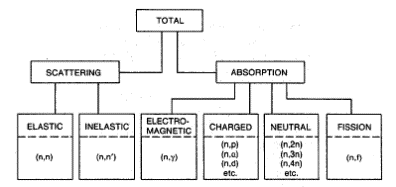
\includegraphics[scale=0.85]{image1.png}\\
\end{center}
L'angle $\alpha$ représenté sur le schéma ci-dessus évoluera jusqu'à un angle limite :
$$\alpha_{lim} = arctg(\frac{T_{lim}}{N})$$
Il s'agit de la \textit{loi de frottement statique}. On remarque qu'au delà d'un certain $W_{lim}$ le bloc se met à glisser et $T$ (la force de frottement) va descendre subitement pour rester ensuite relativement constante.\\

\begin{center}
	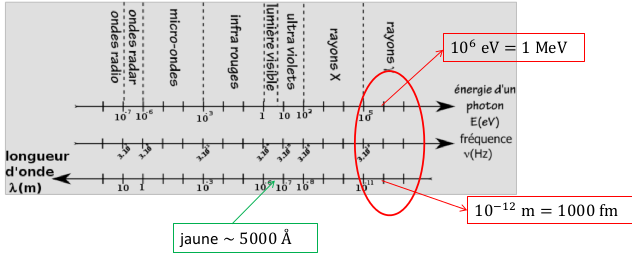
\includegraphics[scale=0.85]{image2.png}\\
\end{center}
Notons que seule la zone $(2)$ et $(4)$ dépendent de la vitesse. La zone $(3)$ représente le frottement lorsque le 'bloc' est en mouvement : \textit{loi de frottement dynamique}. La zone $(4)$ représente les frottements visqueux.\\\\
De façon générale, on peut définir le frottement :
$$T \leq f_{o}N$$
Ou $f_{o}$ est le coefficient de frottement statique. On parlera de frottement dynamique quand :
$$T = f N$$
\ \\
Un cas un peu plus spécial est celui du \textit{basculement}.\\
\begin{center}
	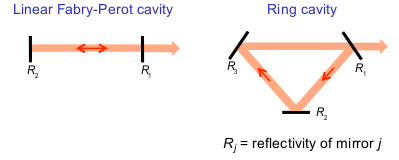
\includegraphics[scale=0.85]{image3.png}\\
\end{center}
A partir d'un certain angle $\alpha$, le bloc ne va pas glisser mais basculer (C'est à dire que la réaction normale au point B sera nulle ($N_{B} = 0$).\\\\
La condition de non basculement vaut ainsi :
$$tg(\alpha) = \frac{a}{h}$$
\ \\ \\

Un dernier cas (promis!) pour la route : le \textit{frottement de roulement}\\
\begin{center}
	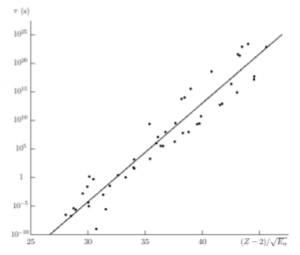
\includegraphics[scale=0.85]{image4.png}\\
\end{center}
On sait déjà (voir un peu plus haut, feignant !) que la sphère ne se met pas à \textbf{glisser} tant que :
$$T_{I} \leq f_oN_1$$
L'expérience montre aussi quelle ne se met pas à \textbf{rouler} tant que :
$$T_{I} \leq kN_1$$
où $k$ est appellé le \textit{coefficiant de roulement statique} (ne dépend que de la nature des matériaux en contact).\\\\
Pour exprimer ça en fonction de $\alpha$, la sphère ne se mettra pas à rouler tant que :
$$\alpha_{max} = arctg(\frac{k}{R})$$

\subsection*{Cas des systèmes plan}
Dans le cas général du plan, si l'appui en un point $A$ laisse au solide $l$ degrés de liberté, ou $l \leq 3$, il faudra introduire en $A r$ composantes de réactions de liaisons et nous auront toujours :
$$l + r = 3$$

\subsection*{Types d'appuis}
\emph{Encastrement}\\\\
\begin{center}
	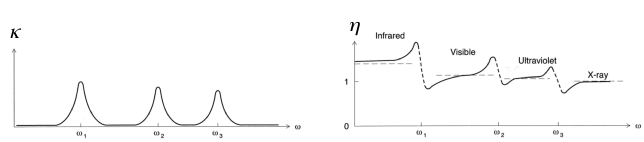
\includegraphics[scale=0.85]{image5.png}\\
\end{center}

\emph{Articulation / rotule}\\\\
\begin{center}
	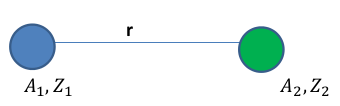
\includegraphics[scale=0.85]{image6.png}\\
\end{center}

\emph{Rouleau}\\\\
\begin{center}
	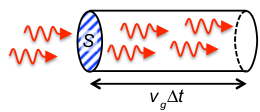
\includegraphics[scale=0.85]{image7.png}\\
\end{center}

\emph{Encastrement à glissière}\\\\
\begin{center}
	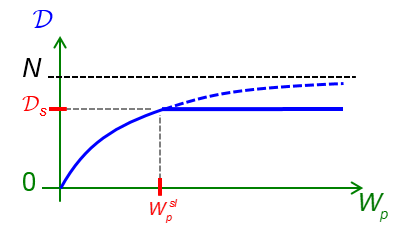
\includegraphics[scale=0.85]{image8.png}\\
\end{center}

\subsection{Systèmes isostatiques, hyperstatiques, hypostatiques}
\begin{itemize}
	\item \textbf{Isostatique :} Si toutes les inconnues peuvent être déterminées par les conditions d'équilibre, et ce, indépendamment des forces agissant sur le solide.\\
	      
	\item \textbf{Hyperstatique :} S'il y a un ou plusieurs degrés de liaisons excédentaires, de sorte que le système des conditions d'équilibre est indéterminé.\\
	      
	\item \textbf{Hypostatique :} S'il manque un ou plusieurs degrés de liaisons pour assurer l'équilibre du solide.\\
	      
	      \subsection{Cas des systèmes spatiaux}
	      Comme pour le plan, mais en 3D ! On a donc :
	      $$l + r =6$$
\end{itemize}

\subsection{Liaison avec le monde extérieur par l'intermédiaire d'un ressort}
L'équation est toujours la même, et est toujours vraie :
$$F = -k \Delta l = -k(l-l_0)$$

\newpage
\chapter{Statique des systèmes de solides}
Les théorèmes généraux sont également en application dans le cas des systèmes de solides. \\\\
Il n'y a rien de spécial à rajouter si ce n'est de tenir compte du principe d'\textit{action/réaction} quand on 'casse' un système en sous-systèmes.\\\\
\textit{NB :} Ne pas hésiter à utiliser les moments de force, c'est souvent simplificateur.

\section{Principe des travaux virtuels}
\subsection{Équilibre d'un point matériel}
Pour tout déplacement virtuel d'un point matériel à partir d'une position d'équilibre, la somme des travaux virtuels effectués par toutes les forces agissant sur le point vaut zéro.\\\\

L'idée est faire un "mini" déplacement faisant \textit{travailler} uniquement les forces qui nous intéressent, en respectant les réactions de liaisons. \\\\
Le principe suivant (décris ci-dessus) nous permet d'avoir une relation nous permettant de lever les inconnues :
$$\delta \tau = \vec{F}. \vec{\delta r} = 0\ \ \ \forall \vec{\delta r}$$

Avant de démontrer ce principe, énonçons avant tout le bien connu \textit{Théorème de Chasles}, mais sous la forme vectorielle !\\
\begin{center}
	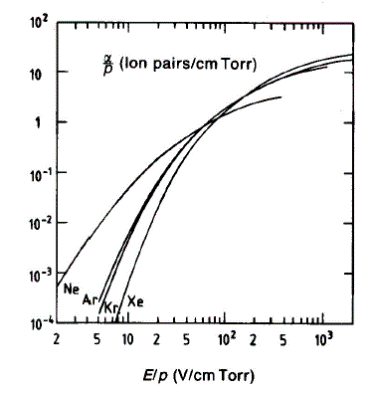
\includegraphics[scale=0.85]{image9.png}\\
\end{center}
$$\overrightarrow{BB'} = \overrightarrow{AA'} + \vec{e}\delta\theta\times\overrightarrow{AB}$$
Nous sommes maintenant armés pour démontrer le principe des travaux virtuels ! \\
\begin{proof}
	\ \\
	Soit les forces de liaisons $L_i$, les forces appliquées $F_i$ telles que : $\vec{R} = \sum_{n} \vec{F_i} + \sum_p \vec{L_i}$.\\
	Le travail virtuel vaut donc :
	$$\delta\tau = \sum_n \vec{F_i} \delta\vec{OP_i}  + \sum_p \vec{L_i} \delta\vec{OQ_i}  $$
	$$\delta\tau = \sum_n \vec{F_i}(\delta\vec{OA} + \vec{e}\delta\theta\times\vec{AP_i}) + \sum_p \vec{L_i}(\delta\vec{OA} + \vec{e}\delta\theta\times\vec{AQ_i})$$
	$$\delta\tau = \sum_n \vec{F_i}\delta\vec{OA} + \sum_n \vec{F_i}(\vec{e}\delta\theta\times\vec{AP_i}) + \sum_p \vec{L_i}\delta\vec{OA} + \sum_p \vec{L_i}(\vec{e}\delta\theta\times\vec{AQ_i})$$
	$$\delta\tau = \delta\vec{OA}\underbrace{[\sum_n \vec{F_i} + sum_p \vec{L_i}]}_{\vec{R}} + \vec{e}\delta\theta\ \underbrace{[\sum_n(\vec{AP_i}\times\vec{F_i}) + \sum_p(\vec{AQ_i}\times\vec{L_i})]}_{\vec{C}} = \vec{0}$$
	On a donc :
	$$\left\lbrace
	\begin{array}{ccc}
		\vec{R} & = & \vec{0} \\
		\vec{C} & = & \vec{0} \\
	\end{array}\right.
	$$
\end{proof}
\textit{NB :} Une coupe travaille uniquement lors d'une rotation, PAS lors d'une translation.

\section{Treillis articulés}
Il s'agit d'un système de barre reliés à leurs extrémités par des articulations (= \textit{nœuds}) formant des mailles indéformables.
\subsection{CN d'isosaticité}
Soit :
\begin{itemize}
	\item[a] : Le nombre de réactions d'appui
	\item[b] : Le nombre de barre du treillis
	\item[n] : Le nombre de nœuds du treillis
\end{itemize}
\ \\
La CN d'isostaticité s'exprime :
$$a + b = 2n$$
On peut dès lors dire que si $a+b > 2n$, le treillis est \textit{hyperstatique}. Si $a+b < 2n$, le treillis est \textit{hypostatique}.\\\\

La plupart des treillis sont hyperstatiques car même si une barre venait à se rompre, le système reste en équilibre. (Typiquement les ailes d'avions).

\section{Potentiel d'un champ de forces conservatif}
\subsection{Champ de forces} 
Il existe deux types de champ de force : central et uniforme :\\\\
\textbf{Champ dit uniforme} : Si a tout point $P$ de sont domaine de définition est associé un vecteur force constant.\\\\
\textbf{Champ dit central} : S'il existe dans son domaine dé définition un point $O$, appelé centre, tel que pour tout point $P$ de ce domaine, $\vec{F}(P)$ ait la direction de $\vec{OP}$.

\subsection{Champ de forces conservatif}
Le travail du champ de forces $\vec{F}(P)$ lors d'un \textit{déplacement quelconque} de son tpoints d'application $P$ le long d'un arc de courbe $AB$ est l'intégrale curviligne, le long de $AB$ :
$$ \tau = \int_A^B \vec{F}(P) . \vec{dr} $$
Les unités du travail sont : $[\tau] = ML^2T^{-2}$. \\
Pour calculer ce genre d'intégrale, ré-ouvrez votre cours de \textit{Connaissances Fondamentales} !\\\\
\emph{Champ conservatif}\\\\
Un champ de force $\vec{F}(P)$ est dit conservatif si le travail le long d'un arc de courbe $AB$ est indépendant du chemin suivi.

\subsection{Potentiel d'un champ de forces conservatif}
\emph{Définition} !\\\\
$$-\tau = - \int_A^B \vec{F}(P) . \vec{dr} = V(B) - V(A)$$
où $ V(B) - V(A)$ est appelée \textit{différence de potentiel entre $B$ et $A$}.

\emph{Potentiel en un point P}\\\\
Celui-ci est défini à un constante près de la façon suivante :
$$V(Q) = - \int_O^Q \vec{F}(P) . \vec{dr}$$

On dira que $\vec{F}(P)$ est conservatif $\Leftrightarrow \vec{F}(P)$ "\textit{dérive d'un potentiel}" (scalaire) $V(P)$.
$$ \Leftrightarrow \vec{F} = -\overrightarrow{grad}\ V = -\vec{\nabla} V$$
où $\vec{\nabla}$ n'est que l'opérateur vectoriel \textit{gradient}. (\textit{cf. Physique Générale et Analyse I})\\

\emph{CS de conservativité d'un champ de forces}\\\\
Cette condition suffisante s'exprime :
$$\exists V\ |\ -\overrightarrow{grad}\ V  \Leftrightarrow \overrightarrow{rot}\ \vec{F} = \vec{0}$$
où $\overrightarrow{rot}$ définit l'opérateur vectoriel \textit{rotationnel}. Celui-ci s'exprime, en coordonnées cartésiennes : 
$$\overrightarrow{rot} = \overrightarrow{grad}\ \times = \vec{\nabla}\ \times$$
Le rotationnel est défini différemment en coordonnées cylindriques et sphériques : \textit{Cf. Analyse I, Ch. 10}. Il ne faut pas les étudier par cœur, une fiche récapitulative sera fournie durant l'examen.\\\\

\textbf{Attention :}  Il faut faire attention au signe de certains champs (\textit{Champ de pesanteur, gravitationnel, ressort linéaire, ...} du à la définitions des axes.

\subsection{Stabilité d'une position d'équilibre}
Un équilibre peut être \textit{stable, instable} ou \textit{indifférent}.
\begin{itemize}
	\item \textbf{Stable :} $\Leftrightarrow \forall$ position voisine (compatible avec les liaisons) : les forces d'action tendent à ramener le corps vers cette position d'équilibre.
	\item \textbf{Instable :} $\Leftrightarrow \exists$ position voisine (compatible avec les liaisons) : les forces d'action tendent à écarter davantage le corps de cette position d'équilibre.
	\item \textbf{Indifférent :} $\Leftrightarrow \forall$ position voisine (compatible avec les liaisons) : 
	      le corps reste dans cette nouvelle position sous l'effet des forces d'action.
\end{itemize}\ \\
\textbf{Attention :} Il s'agit bien d'un $\exists$ pour le deuxième cas, et non d'un $\forall$.\\\\

\emph{Critère de stabilité}\\\\
Théorème de Lejeune-Dirichlet :
\begin{center}
	\textit{Une position d'équilibre d'un point matériel est stable si et seulement si le potentiel de la résultante des forces d'action est minimum dans cette position.}
\end{center}\ \\
Trois cas sont à considérer : 
\begin{enumerate}
	\item $\frac{d^2V}{du}|_{u^*} > 0$ $V(u)$ est minimum en $u=u^* \Rightarrow$ \textbf{Équilibre stable}.
	\item $\frac{d^2V}{du}|_{u^*} < 0$ $V(u)$ est maximum en $u=u^* \Rightarrow$ \textbf{Équilibre instable}.
	\item $\frac{d^2V}{du}|_{u^*} = 0$ $V(u)$ est constante $\Rightarrow$ \textbf{Équilibre indifférent}.
\end{enumerate}\ \\
\begin{center}
	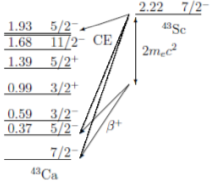
\includegraphics[scale=0.85]{image10.png}\\
\end{center}

\newpage
\chapter{Cinématique du point}
\section{Objet le a cinématique}
La \textbf{cinématique} décrit les mouvements d'un système de points en introduisant un nouveau concept fondamental : le temps.
\section{Trajectoire d'un point}
Soit ${O; \vec{1_x}, \vec{1_y}, \vec{1_z})}$ un repère fixe constitué d'un point de référence $O$ et soit $E = [t_0, t_f]$ un intervalle te temps tel que $t_0 < t < t_f$.\\
La loi de mouvement de P par rapport au repère (où $\vec{OP}$ est le vecteur position) se définit par : 
$$\vec{OP}(t) = \vec{r}(t) = x(t)\vec{1_x} + y(t)\vec{1_y} + z(t)\vec{1_z}$$
Les lieux des points successivement occupés par $P$ lorsque $t$ prend ses valeurs dans l'intervalle $I$ est appelé \textbf{trajectoire de P}.\\
\textit{NB :} Le sens de parcours correspond à celui d'un $t$ croissant.

\section{Vitesse d'un point}
\subsection{Définition}
La \textbf{vitesse} d'un point P dans le repère fixe ${O; \vec{1_x}, \vec{1_y}, \vec{1_z})}$ à l'instant $t^*$ est la dérivée de $\vec{r}(t)$ par rapport à $t$ à l'instant $t^*$ :
$$\vec{v(t^*)} = \frac{d\vec{r}(t)}{dt}\mid_{t=t^*}$$
\textit{NB :} Pour une dérivée par rapport au temps, on introduit la  notation : $\dot{\ } = \frac{d}{dt}$
\subsection{Composantes cartésiennes}
$$ \vec{v}(t) = \dot{x}(t)\vec{1_x} + \dot{y}(t)\vec{1_y} + \dot{z}(t)\vec{1_z}$$

\subsection{Composantes intrinsèques (Trièdre de Frenet)}
Le \textbf{repère intrinsèque} de Frenet est constitué d'une base orthonormée : 
$$\left( \vec{1_t}(u), \vec{1_n}(u), \vec{1_b}(u)\right)$$

Il faut d'abord trouver le vecteur unitaire tangent :
$$\vec{1_t} = \frac{d\vec{r}}{ds}$$
où $s$ représente la longueur de l'arc de la courbe entre un point origine et le point.\\

Le vecteur binormal, lui, se définit :
$$\vec{1_b} = \vec{1_t} \times \vec{1_n}$$
Pour le vecteur normal ($\vec{1_n}$), on essaye de le trouver (en méca) par  la géométrie. Dans le plan, c'est toujours $\pm \vec{1_z}$.\\

\textbf{Expression du vecteur vitesse}\\
$$\vec{v} = \dot{s}(y)\vec{1_t}$$
\textit{Cf. cours de géométrie pour plus de détails}

\subsection{Composantes polaires et cylindriques}
\textbf{Vecteur de Darboux d'une base orthonormée mobile}\\
En passant les détails technique, le(s) vecteur(s) de Darboux s'expriment :
$$\frac{d\vec{E}_i}{dt} = \omega \times \vec{E}_i$$

\textbf{Vecteur de Darboux de la base des coordonnées cylindriques}\\
Il est \textbf{très important} de savoir retrouvé ce vecteur de soi même! Je ne mets ici que le résultat final, mais c'est important de les retrouver seuls!
$$\vec{\omega} = \dot{\theta}\vec{1_z}$$

\textbf{Vecteur de Darboux de la base de coordonnée sphériques}\\
En toute généralité, un vecteur rotation permettant le passage d'une base (cartésienne pour faire simple) vers (ici) la base de coordonnée sphérique.\\
Encore une fois, je mets le résultat mais celui-ci \textbf{doit} savoir être trouvé seul !
$$\vec{\omega} = \dot{\phi}cos\theta\vec{1_r} - \dot{\phi}sin\theta \vec{1_\theta} + \dot{\theta}\vec{1_\phi}$$
\begin{center}
	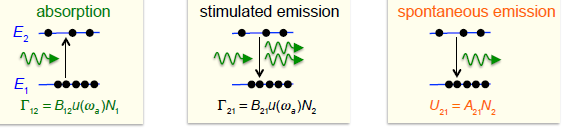
\includegraphics[scale=0.85]{image11.png}\\
\end{center}
\textit{Le graphique ci-dessus représente la composée d'une rotation d'angle $ \phi$ autour de $Oz$ et une deuxième d'angle $\theta$ autour de l'axe $Oy_1$ tout comme le fait $\vec{\omega}$}.\\

\textbf{Dérivées d'une fonction vectorielle exprimée par ses composantes dans une base orthonormée mobile}\\
\textit{Cf. page 88 - 89}

\subsection{Composantes polaires et cylindriques de la vitesse}
\emph{Base des coordonnées polaires : $(\vec{1_r}(\theta), \vec{1_\theta}(\theta)$}\\\\
Le déplacement en coordonnée polaire s'exprime : 
$$\vec{dr} = dr\vec{1_r} + rd\theta\vec{1_\theta}$$
On peut en tirer le vecteur vitesse : 
$$\vec{v}(t) = \dot{r}\vec{1_r} + r\dot{\theta}\vec{1_\theta}$$
\ \\
\emph{Base des coordonnées cylindrique : $(\vec{1_r}(\theta), \vec{1_\theta}(\theta), \vec{1_z}$}\\\\
Le déplacement en coordonnée cylindrique s'exprime : 
$$\vec{dr} = dr\vec{1_r} + rd\theta\vec{1_\theta} + dz\vec{1_z}$$
On peut en tirer le vecteur vitesse : 
$$\vec{v}(t) = \dot{r}\vec{1_r} + r\dot{\theta}\vec{1_\theta} + \dot{z}\vec{1_z}$$

\subsection{Composantes sphériques de la vitesse}
\emph{Base des coordonnées sphérique : $(\vec{1_r}(\theta, \phi), \vec{1_\theta}(\theta, \phi), \vec{1_\phi}(\phi)$}\\\\
Le déplacement en coordonnée cylindrique s'exprime : 
$$\vec{dr} = dr\vec{1_r} + rd\theta\vec{1_\theta} + rin\theta d\phi\vec{1_\phi}$$
On peut en tirer le vecteur vitesse : 
$$\vec{v}(t) = \dot{r}\vec{1_r} + r\dot{\theta}\vec{1_\theta} + r sin\theta\dot{\phi} \vec{1_\phi}$$

\section{Accélération d'un point}
\subsection{Définition}
L'\textbf{accélération} du point $P$ à l'instant $t$ est la dérivée de $\vec{v}(t)$ :
$$\vec{j}(t) = \frac{d\vec{v}(t)}{dt}$$

\subsection{Composantes cartésiennes}
$$\vec{j}(t) = \ddot{x}(t) \vec{1_x} + \ddot{y}(t)\vec{1_y} + \ddot{z}(t)\vec{1_z}$$

\subsection{Composantes intrinsèques (Frenet)}
$$\vec{j}(t) = \underbrace{(\vec{J}_t.\vec{1_t})}_{J_t}.\vec{1_t} + \underbrace{(\vec{J}_n.\vec{1_n})}_{J_n}.\vec{1_n}$$
La torsion se calcule :

\subsection{Composantes polaires et cylindriques}
\textit{Cf. page 94}

\subsection{Composantes sphériques}
\textit{Cf. page 94}

\section{Applications à des mouvements particuliers}
\subsection{Mouvement rectiligne}
Rappel du secondaire. J'énonce simplement la formule complète :
$$\vec{OP}(t) = \vec{r}(t) = (x + \dot{x}t + \frac{1}{2}\ddot{x}t^2)\vec{1_x}$$

\subsection{Mouvement circulaire}
$$\vec{v}(t) = \omega R \vec{1_\theta}$$
$$\vec{j}(t) = -\omega^2 R \vec{1_r} + \epsilon R \vec{1_\theta}$$
où $\epsilon$ est l'accélération angulaire.

\section{Mouvement relatif d'un point}
\subsection{Trajectoire absolue, relative et d'entraînement}
Considérons un repère $Oxyz$ \textbf{absolu} et un reprère mobile $O'XYZ$, de vecteur de Darboux $\vec{\omega}(t)$ par rapport à Oxyz que nous désignerons pas \textbf{repère relatif}. Définissons trois trajectoire possible : 
\begin{enumerate}
	\item \textbf{Absolue} : Lieu de points de l'espace successivement occupés par $P$ pour un observateur attaché au repère fixe $Oxyz$.
	\item \textbf{Relative} : Lieu de points de l'espace successivement occupés par $P$ pour un observateur attaché au repère fixe $O'XYZ$.
	\item \textbf{Entraînement} : Lieu des points de l'espace qu'occuperait successivement $P$ pour un observateur attaché au repère $Oxyz$ s'il était fixé dans les axes relatif $O'XYZ$.
\end{enumerate}
\begin{center}
	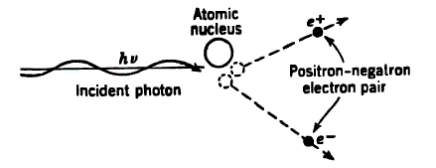
\includegraphics[scale=0.65]{image12.png}\\
\end{center}

\subsection{Théorème de Coriolis}
\textbf{Premier théorème de Coriolis}\\
Celui-ci concerne les vitesses.
\begin{itemize}
	\item $\vec{v}_{abs} = \vec{v}_{rel} + \vec{v}_{entr}$
	\item $\vec{v}_{rel}$ = $\frac{d\vec{O'P}}{dt}|_{rel}$
	\item $\vec{v}_{entr}$ =  $\vec{v}_{O'} + \vec{\omega}\times\vec{O'P}$
\end{itemize}
\ \\

\textbf{Second théorème de Coriolis}\\
Celui-ci concerne les accélérations.

\subsection{Application : équilibre relatif d'un point matériel}
\begin{itemize}
	\item $\vec{j}_{abs} = \vec{j}_{rel} + \vec{j}_{entr} + \vec{j}_{cor}$
	\item $\vec{j}_{rel}$ = $\frac{d^2\vec{O'P}}{dt^2}|_{rel} = \frac{d\vec{v}_{rel}}{dt}$
	\item $\vec{j}_{entr}$ =  $\vec{j}_{O'} + \vec{\epsilon}\times \vec{O'P} + \vec{\omega}(\vec{\omega}\times\vec{O'P})$
\end{itemize}
où $\vec{\epsilon}(t)$ est la dérivée de $\vec{\omega}(t)$ par rapport au temps.
\newpage
\chapter{Dynamique du point}
\$

%%%%%%%%%%%%%%%%%
% Bibliographie %
%%%%%%%%%%%%%%%%%
%\newpage
%\chapter{Bibliographie}
%\nocite{*}
%\printbibliography[heading=none]

%%%%%%%%%%%
% Annexes %
%%%%%%%%%%%
\appendix
%\input{annexes/annexe1.tex}


\end{document}


